\section{Programación Lineal}

\subsection{Introducción}

La programación lineal es una técnica matemática de optimización que se utiliza para encontrar la mejor solución posible a un problema cuando se tienen recursos limitados y múltiples opciones para usar esos recursos.

¿Qué es exactamente? Es un método que permite maximizar o minimizar una \hl{función objetivo} (como ganancias, costos, tiempo, etc.) sujeta a un conjunto de \hl{restricciones lineales}. Tanto la función objetivo como las restricciones se expresan mediante ecuaciones o inecuaciones lineales, es decir, donde las variables aparecen elevadas solo a la primera potencia.

\noindent\textbf{Componentes principales:}
\begin{itemize}
  \item \textbf{Función objetivo}: Lo que queremos optimizar (maximizar ganancias o minimizar costos, por ejemplo)
  \item \textbf{Variables de decisión}: Las cantidades que podemos controlar y necesitamos determinar
  \item \textbf{Restricciones}: Las limitaciones del problema (presupuesto disponible, tiempo, materiales, capacidad de producción, etc.)
\end{itemize}

\subsection{Problemas de Optimización}

En un \textit{problema de optimización}, se busca maximizar o minimizar una cantidad específica llamada \hl{objetivo}, la cual depende de un número finito de variables de entrada. Estas variables pueden ser independientes entre sí o estar relacionadas a través de una o más restricciones.

\ejemplo\label{ej:ppl_lineal}: El siguiente problema:
\begin{align*}
  \text{max:} \quad         &z = 3x_1 + 2x_2 \\[3pt]
  \text{sujeto a:} \quad    &x_1 + x_2 \leq 10 \\
                            &x_1,x_2 \geq 0
\end{align*}
es un problema de optimización para el objetivo \(z\). Las variables de entrada son \(x_1\) y \(x_2\) y se denominan \textit{variables de decisión}, que deben cumplir dos restricciones: \(x_1 + x_2 \leq 10\) y \(x_1,x_2 \geq 0\).

El problema del ejemplo \ref{ej:ppl_lineal} pide maximizar \(z = 3x_1 + 2x_2\), es decir, encontrar los valores de \(x_1\) y \(x_2\) que maximicen \(z\) bajo las restricciones dadas.

En general, se llama PPL a un problema de optimización que se puede resolver mediante técnicas de programación lineal. Un problema de programación matemático es lineal si tanto la función objetivo \(z\) como las restricciones son lineales. Esto es:
\begin{align*}
  \text{optimizar:} \quad         &z = f(x_1, x_2, \ldots, x_n) \\[3pt]
  \text{sujeto a:} \quad    &g_i(x_1, x_2, \ldots, x_n) \thicksim  b_i \qquad \forall i \in \{1, 2, \ldots, m\} \\
\end{align*}
donde las restricciones son ecuaciones o desigualdades lineales, es decir emplean alguno de los símbolos \(\leq\), \(\geq\) o \(=\).

\subsection{Planteamiento de problemas}

Los problemas de optimización se plantean muy a menudo verbalmente, es decir, en palabras. Ya se verá un ejemplo a continuación (ejemplo \ref{ej:ppl_verbal}) de un problema de optimización planteado verbalmente. El procedimiento para la solución consiste en realizar un modelo del problema para poder resolverlo mediante técnicas de programación lineal.

\begin{tcolorbox}[interesting_data, title=¿Existe solo una forma de plantear problemas?]
  Existen múltiples formas de plantear un problema de optimización, por lo que los dos métodos que se proponen en este documento puedes tomarlos como sugerencias.
\end{tcolorbox}

\ejemplo\label{ej:ppl_verbal}: Una compañía de petróleos produce en sus refinerías gasóleo (\(G\)), gasolina sin plomo (\(P\)) y gasolina súper (\(S\)) a partir de dos tipos de crudos, \(C_1\) y \(C_2\). Las refinerías están dotadas de dos tipos de tecnologías. La tecnología nueva (\(T_n\)) utiliza en cada sesión de destilación \(7\) unidades de \(C_1\) y \(12\) de \(C_2\), para producir \(8\) unidades de \(G\), \(6\) de \(P\) y \(5\) de \(S\). Con la tecnología antigua (\(T_a\)), se obtienen en cada destilación \(10\) unidades de \(G\), \(7\) de \(P\) y \(4\) de \(S\), con un gasto de \(10\) unidades de \(C_1\) y \(8\) de \(C_2\).

Estudios de la demanda permiten estimar que para el próximo mes se deben producir al menos \(900\) unidades de \(G\), \(300\) de \(P\) y entre \(800\) y \(1700\) de \(S\). La disponibilidad de \(C_1\) es de \(1400\) unidades y de \(C_2\) de \(2000\) unidades. Los beneficios por unidad producida son:
\begin{table}[ht]
  \centering
  \begin{tabular}{|c|c|c|c|}
  \hline
  Gasolina & \textit{G} & \textit{P} & \textit{S} \\ \hline
  Beneficio/u & 4 & 6 & 7 \\ \hline
  \end{tabular}
\end{table}

La compañía desea conocer cómo utilizar ambos procesos de destilación, que se pueden utilizar total o parcialmente, y los crudos disponibles para que el beneficio sea el máximo.

\vspace{5mm}
\hrule
\vspace{5mm}

Este problema es un ejemplo típico de un PPL verbal. Hay una cantidad que se desea optimizar y un conjunto de restricciones que se deben cumplir. En este caso, se desea maximizar el beneficio y las restricciones son las cantidades de crudos disponibles y las cantidades de gasolina que se deben producir. Más adelante vamos a plantear el PPL asociado a este problema y vamos a resolver otros problemas. De momento con darnos a la idea de cómo es un problema verbal es suficiente.

\subsubsection{Métodos de planteamiento de PPLs}

Como dijimos anteriormente, existen múltiples formas de plantear un problema de optimización, por lo que los dos métodos que se proponen son el método recomendado por el libro Bronson (sacado de la cátedra) y el método que se propone en el libro de Alfaomega (\cite{PPL_Alfaomega}). 

Luego de describir los métodos de planteamiento de PPLs, el ejemplo \ref{ej:modelo_de_ppl_verbal} muestra el planteo del ejemplo \ref{ej:ppl_verbal} con el método de Alfaomega.

\begin{tcolorbox}[title=Método del libro Bronson]
  Luego de tener un enunciado verbal de un problema de optimización, se deben seguir los siguientes pasos:
  \begin{enumerate}
    \item Determínese la cantidad que se optimizará y exprésese como una función matemática. Hacer esto sirve para definir las variables de decisión.
    \item Identifíquese todos los requerimientos, restricciones y limitaciones estipulados, y exprésense matemáticamente. Estos requerimientos constituyen las restricciones.
    \item Exprésense todas aquellas condiciones ocultas. Tales condiciones no están estipuladas explícitamente, pero se hacen evidentes a partir de la situación física para la que se está planteando el modelo. Generalmente, involucran requerimientos de no negatividad o de ser enteras, para las variables de decisión.
  \end{enumerate}  
\end{tcolorbox}

\noindent Por otro lado, el método que se proponen en el libro PPL de Alfaomega es el siguiente:
\begin{tcolorbox}[title=Método del libro Alfaomega]
  \begin{enumerate}
    \item \textit{Reconocimiento de las variables de decisión}: las variables de decisión son las variables sobre las que el decisor tiene control y que se suponen continuas. Representan productos o bienes a producir, almacenar o vender, disponibilidad o adquisición de materias primas, etc.
    \item \textit{Identificación de las restricciones}: las restricciones representan las limitaciones o requisitos y definen la \textit{región factible} del problema. Representan el deseo de no exceder un valor específico (\(\leq\)), no descender por debajo de un valor particular (\(\geq\)) o ser igual a un valor particular (\(=\)).
    \item \textit{Obtención de la función objetivo}: la función objetivo es la que se quiere maximizar o minimizar. Representa el beneficio, renta, ganancias, costos, etc.
    \item \textit{Formulación del PPL}: cuando se tienen los tres pasos anteriores se puede formular el PPL. La solución de este PPL se denomina \textit{solución óptima} y se estudiará en la proxima sección.
  \end{enumerate}
\end{tcolorbox}

\begin{tcolorbox}[mydanger]
  \textbf{Cuidado:} El paso 2 de la metodología de Alfaomega incluye \textit{todas} las restricciones, incluso aquellas que no están en el enunciado verbal (como no negatividad por ejemplo).
\end{tcolorbox}

\vspace{5mm}
\hrule
\vspace{5mm}

\ejemplo\label{ej:modelo_de_ppl_verbal}: Tomemos el PPL verbal del ejemplo \ref{ej:ppl_verbal}. Propongo al lector que intente plantear el PPL asociado (no resolver) y luego comparar con la solución. En este caso vamos a modelar el PPL siguiendo el método recomendado por el libro de Alfaomega (segundo método).

\noindent\textbf{Paso 1: Reconocimiento de las variables de decisión}

Si bien la consigna puede resultar un poco enredada al principio, si prestamos atención, vemos que al final nos pregunta sobre \hl{cómo usar los procesos de destilación}. Esto nos da un indicio de que lo que se quiere es saber cuánto usar el proceso \(T_n\) y el proceso \(T_a\) para maximizar el beneficio.

Entonces, las variables sobre las que el vendedor tiene control son:
\begin{itemize}
  \item \(x_1 ~\rightarrow\) cantidad de sesiones de destilación usando el proceso \(T_n\)
  \item \(x_2 ~\rightarrow\) cantidad de sesiones de destilación usando el proceso \(T_a\)
\end{itemize}

\noindent\textbf{Paso 2: Identificación de las restricciones}

Tenemos restricciones debidas a las limitaciones en la disponibilidad de ambos tipos de crudos:
\begin{itemize}
  \item Para \(C_1\): \(7x_1 + 10x_2 \leq 1400\)
  \item Para \(C_2\): \(12x_1 + 8x_2 \leq 2000\)
\end{itemize}

\noindent También se tienen restricciones según las necesidades de refinado que se requieren:
\begin{itemize}
  \item Para Gasóleo (\(G\)): \(8x_1 + 10x_2 \geq 900\)
  \item Para Sin Plomo (\(P\)): \(6x_1 + 7x_2 \geq 300\)
  \item Para Super (\(S\)): \((5x_1 + 4x_2 \geq 800) \wedge (5x_1 + 4x_2 \leq 1700)\)
\end{itemize}

\noindent Además no debemos olvidar de tener en cuenta las restricciones implícitas, ya que es obvio que no se pueden realizar destilaciones negativas, se tiene:
\begin{itemize}
  \item \(x_1 \geq 0\)
  \item \(x_2 \geq 0\)
\end{itemize}

\noindent\textbf{Paso 3: Identificación de la función objetivo}

El beneficio será la suma de las cantidades de cada refinado que se vende, por lo que:
\begin{itemize}
  \item Cantidad de Gasóleo: \(8x_1 + 10x_2 ~ \rightarrow G \times \text{Precio: } 4(8x_1 + 10x_2) = 32x_1 + 40x_2\)
  \item Cantidad de Sin Plomo: \(6x_1 + 7x_2 ~ \rightarrow P \times \text{Precio: } 6(6x_1 + 7x_2) = 36x_1 + 42x_2\)
  \item Cantidad de Super: \(5x_1 + 4x_2 ~ \rightarrow S \times \text{Precio: } 7(5x_1 + 4x_2) = 35x_1 + 28x_2\) 
\end{itemize}

\noindent Por lo tanto, la función objetivo es:
\begin{align*}
  z &= 32x_1 + 40x_2 + 36x_1 + 42x_2 + 35x_1 + 28x_2 \\
    &= 103x_1 + 110x_2
\end{align*}

\noindent\textbf{Paso 4: Formulación del PPL}
\begin{align*}
  \text{maximizar:} \quad   &z = 103x_1 + 110x_2 \\[3pt]
  \text{sujeto a:} \quad    &7x_1 + 10x_2 \leq 1400 \\
                            &12x_1 + 8x_2 \leq 2000 \\
                            &8x_1 + 10x_2 \geq 900 \\
                            &6x_1 + 7x_2 \geq 300 \\
                            &5x_1 + 4x_2 \geq 800 \\
                            & 5x_1 + 4x_2 \leq 1700 \\
                            &x_1 \geq 0 \\
                            &x_2 \geq 0
\end{align*}

Es muy importante entender la metodología del planteo, ya que si el modelo realizado no es adecuado, el resultado obtenido cuando se resuelva el problema será, muy probablemente, incorrecto.

Al intentar plantear el problema del ejemplo \ref{ej:ppl_verbal} tal vez te hayan surgido algunas dudas, así que vamos a realizar un pequeño repaso sobre algunos detalles en el procedimiento del ejemplo \ref{ej:modelo_de_ppl_verbal}.

\noindent\textbf{¿Por qué se tomaron \(T_n\) y \(T_a\) como variables de decisión y no \(C_1\) y \(C_2\)?}

Tal vez podrías pensar que \(C_1\) y \(C_2\) pueden ser buenos candidatos a variables de decisión, ya que el vendedor puede controlar cuánta cantidad de cada tipo de curdo usa en cada tecnología. Entonces intentemos generar un modelo con \(C_1\) y \(C_2\) como variables de decisión.

Como ya sabemos que las variables de decisión son \(C_1\) y \(C_2\) entonces el paso 1 resulta:
\begin{itemize}
  \item \(x_1 ~\rightarrow\) cantidad de crudo \(C_1\) utilizado
  \item \(x_2 ~\rightarrow\) cantidad de crudo \(C_2\) utilizado
\end{itemize}

\noindent En el paso 2 tenemos las restricciones:
\begin{enumerate}
  \item Según la tecnología usada
  \item Según la cantidad de crudo disponible
  \item Según la cantidad de refinado que se debe producir dependiendo de la tecnología usada
  \item Restricción de no negatividad (no se pueden refinar cantidades negativas)
\end{enumerate}
Si bien de alguna forma rebuscada puede llegarse a un PPL equivalente, vemos que es mucho más complicado, ya que la tercer restricción está relacionando los crudos con el destilado y la tecnología, por lo que serán restricciones largas y complejas de modelar correctamente.

Es de mucha importancia tomarse el tiempo de analizar bien cuáles son las variables de decisión, ya que de ahí partirá todo el modelo. En caso de que usted elija utilizar el procedimiento de formulación de modelos del libro de Bronson, el paso 1 tiene este riesgo implícito, ya que si se genera una función objetivo cuyas variables de decisión no sean las adecuadas, el modelo puede terminar por ser incorrecto.

En este documento se ha usado el enfoque de Alfaomega ya que la idea de tener un paso específico para analizar el enunciado y tomar las variables de decisión es muy importante y no debe pasarse por alto.

\subsection{Resolución de Programas Lineales}

En esta materia se ven dos métodos para resolver PPLs:
\begin{itemize}
  \item \textbf{Método Gráfico}: se basa en la representación gráfica de las restricciones y de la solución. Tiene la ventaja de ser muy intuitivo y sencillo de entender, pero tiene la desventaja de ser poco eficiente y muy limitado en cuanto al número de variables.
  \item \textbf{Método Analítico}: Es más general que el método gráfico ya que no tiene la desventaja de límite de variables. Este método se conoce como el método Simplex y es muy eficiente y algorítmico. La desventaja es que requiere la transformación previa al \textit{formato estándar} añadiendo variables de holgura y/o variables artificiales.
\end{itemize}
Más adelante veremos en profundidad los dos métodos, así que no se preocupe por el vocabulario desconocido.

\subsubsection{Típos de solución}

Todo PPL puede tener alguna de las siguientes soluciones:
\begin{itemize}
  \item Solución optima única
  \item Solución optima múltiple
  \item Problema no acotado
  \item Problema infactible
  \item Rayo óptimo
\end{itemize}

A continuación vamos a profundizar un poco sobre qué significa cada tipo de solución, para que al momento de resolver PPLs sepa identificar qué tipo de solución tiene.

\paragraph{Solución óptima única}

\noindent Es el caso más común y deseable. Existe exactamente un punto en la región factible donde la función objetivo alcanza su valor óptimo (máximo o mínimo) y presenta las siguientes características:
\begin{itemize}
  \item La función objetivo tiene una pendiente única que no es paralela a ninguna cara de la región factible
  \item Gráficamente, la línea de la función objetivo ``toca'' la región factible en un solo vértice
  \item Matemáticamente, existe un único vector \(x^*\) que optimiza la función
\end{itemize}

\paragraph{Solución óptima múltiple (infinitas soluciones óptimas)}

Existen infinitos puntos que proporcionan el mismo valor óptimo de la función objetivo. Esto ocurre cuando:
\begin{itemize}
  \item La función objetivo es paralela a una de las caras (aristas) de la región factible
  \item Todos los puntos en esa arista proporcionan el mismo valor óptimo
\end{itemize}
Este tipo de soluciones tienen las siguientes características:
\begin{itemize}
  \item Cualquier combinación convexa de dos vértices óptimos adyacentes también es óptima
  \item La solución es un segmento de línea completo en la frontera de la región factible
\end{itemize}

Si el problema tiene una solución óptima múltiple, entonces no existe una preferencia por una solución sobre otra, ya que todas son óptimas. La respuesta que usted elija darle al problema será cualquiera de las soluciones óptimas, y será considerada correcta.

\paragraph{Problema no acotado}

La función objetivo puede crecer (o decrecer) indefinidamente sin violar ninguna restricción. Estos problemas presentan las siguientes características:
\begin{itemize}
  \item La región factible se extiende infinitamente en la dirección que mejora la función objetivo
  \item No existe un valor máximo (o mínimo) finito para la función objetivo
  \item Indica generalmente un error en la formulación del problema
\end{itemize}

\ejemplo : Maximizar \(z = x_1 + x_2\) sujeto solo a \(x_1 \geq 0, x_2 \geq 0\) (sin restricciones superiores).

\paragraph{Problema infactible}

No existe ningún punto que satisfaga simultáneamente todas las restricciones del problema. Este tipo de problemas pueden ocurrir en dos casos:
\begin{itemize}
  \item Las restricciones son contradictorias entre sí
  \item El conjunto de restricciones no tiene intersección común
\end{itemize}
Y presentan las siguientes características:
\begin{itemize}
  \item La región factible está vacía
  \item No hay solución posible al problema
  \item Matemáticamente: el conjunto \(\{x : Ax \leq b, x \geq 0\} = \emptyset\)
\end{itemize}

\ejemplo : Sea el siguiente PPL:
\begin{align*}
  \text{maximizar:} \quad   &z = x_1 + x_2 \\[3pt]
  \text{sujeto a:} \quad    &x_1 + x_2 \leq 5 \\
                            &x_1 + x_2 \geq 10 \\
                            &x_1, x_2 \geq 0
\end{align*}
Estas restricciones son imposibles de satisfacer simultáneamente.

\paragraph{Rayo óptimo}

Este es un caso especial del problema no acotado donde existe una dirección específica (rayo) a lo largo de la cual la función objetivo mejora indefinidamente. Este tipo de problemas presentan las siguientes características:
\begin{itemize}
  \item Existe un punto factible \(x_0\) y una dirección \(d\) tal que \(x_0 + \lambda d\) es factible para todo \(\lambda \geq 0\)
  \item La función objetivo mejora a lo largo de esta dirección: \(c^T d > 0\) (para maximización)
  \item El rayo representa la dirección de crecimiento ilimitado
\end{itemize}
La diferencia con la solución de tipo ``no acotado'' es que el rayo óptimo especifica exactamente la dirección del crecimiento infinito, mientras que ``no acotado'' es la conclusión general.

\paragraph{Identificación en el método simplex}

En el método simplex, la identificación de los tipos de soluciones se realiza de la siguiente manera:
\begin{itemize}
  \item \textbf{Única/Múltiple:} Se identifica en la tabla final del simplex
  \item \textbf{No acotado:} Aparece cuando una variable no básica tiene coeficientes no positivos en su columna
  \item \textbf{Infactible:} Se detecta cuando aparecen variables artificiales con valor positivo en la solución final
  \item \textbf{Rayo óptimo:} Se determina por la dirección correspondiente a la variable que causa el comportamiento no acotado
\end{itemize}

Cada tipo de solución tiene implicaciones importantes para la interpretación y aplicación práctica del modelo de optimización. De momento no se preocupe por entender el método simplex, ya que se verá en detalle en la siguiente sección.

\subsubsection{Método Gráfico}

Como se mencionó anteriormente, el método gráfico es muy intuitivo, y por ende, ideal para aprender los conceptos de PPLs. Para entender el método gráfico lo más sencillo es analizarlo con un ejemplo.

\ejemplo\label{ej:mtd_grfico}: Un expendio de carnes de la cuidad acostumbra a preparar carne para albondigón con una combinación de carne molida de res y carne molida de cerdo. La carne de res contiene \(80\%\) de carne y \(20\%\) de grasa, y le cuesta a la tienda \textcent \textit{80} por libra; la carne de cerdo contiene \(68\%\) de carne y \(32\%\) de grasa y cuesta \textcent \textit{60} por libra 

¿Qué cantidad de cada tipo de carne debe emplear la tienda en cada libra de albondigón, si se desea minimizar el costo y mantener el contenido de grasa no mayor al \(25\%\)?

\noindent\textbf{Resolución del ejemplo \ref{ej:mtd_grfico}:}
\begin{quote}
  \textbf{1. Identificación de variables de decisión:}
  Vemos que el resultado es un albondigón, y este se prepara con \(x_1\) libras de carne de res y \(x_2\) libras de carne de cerdo. Por lo que las variables de decisión son:
  \begin{itemize}
    \item \(x_1 ~\rightarrow\) cantidad de carne de res por libra de albondigón
    \item \(x_2 ~\rightarrow\) cantidad de carne de cerdo por libra de albondigón
  \end{itemize}

  \textbf{2. Identificación de restricciones:}
  Vemos que la cantidad total de grasa del albondigón debe ser menor o igual al 25\%, y que la cantidad de carne de res más la cantidad de carne de cerdo debe ser igual a 1 libra.

  Sumado a esto, también se tiene que las cantidades de carne de res y carne de cerdo no pueden ser negativas. Entonces, resulta:

  \begin{align*}
    0.2x_1 + 0.32x_2 &\leq 0.25 \\
    x_1 + x_2 &= 1 \\
    x_1, x_2 &\geq 0
  \end{align*}

  \textbf{3. Identificación de la función objetivo:}

  Vemos que la función objetivo es el costo total, que es la suma del costo de la carne de res y la carne de cerdo. Por lo que la función objetivo es:
  \[
    z = 80x_1 + 60x_2
  \]

  \textbf{4. Formulación del PPL:}

  Juntando la función objetivo con las restricciones, resulta en el siguiente PPL:
  \begin{align*}
    \text{minimizar:} \quad   &z = 80x_1 + 60x_2 \\[3pt]
    \text{sujeto a:} \quad    &0.2x_1 + 0.32x_2 \leq 0.25 \\
                              &x_1 + x_2 = 1 \\
                              &x_1, x_2 \geq 0
  \end{align*}

  \textbf{5. Resolución del PPL:}

  Para resolver el PPL usando el método gráfico, debemos graficar las restricciones, la región factible y la función objetivo. 

  \noindent ¿Cómo se realiza la gráfica de la función objetivo? 

  Para realizar la gráfica de la función objetivo debemos establecer un valor para el costo, y verificar si se encuentra en la región factible. Por ejemplo, nosotros vamos a elegir un valor inicial de \(z = 50\), y resolver la ecuación \(50 = 80x_1 + 60x_2\) para obtener la ecuación de la recta que representa la función objetivo.
  \begin{align*}
    50 &= 80x_1 + 60x_2 \\
    x_2 &= -\frac{4}{3}x_1 + \frac{5}{6}
  \end{align*}
  Y listo, ahora solo debemos graficar las restricciones e identificar la región factible, que la marcaremos de color \textcolor{cyan}{cyan}. 
    
  \begin{figure}[ht]
  \centering
  \begin{tikzpicture}
  \begin{axis}[
      xlabel={$x_1$},
      ylabel={$x_2$},
      xmin=0, xmax=1.5,
      ymin=0, ymax=1.2,
      grid=major,
      axis lines=center,
      legend pos=north east,
      width=10cm,
      height=8cm
  ]

  % Restricción 1: 0.2x1 + 0.32x2 <= 0.25
  \addplot[orange, thick, domain=0:1.25, name path=A] {-(4/7)*x + (5/7)};
  \addlegendentry{\(0.2x_1 + 0.32x_2 \leq 0.25\)}

  % Restricción 2: x1 + x2 <= 1
  \addplot[blue, thick, domain=0:1, name path=B] {1-x};
  \addlegendentry{\(x_1 + x_2 = 1\)}

  % Función objetivo (para un valor de z=50): 50 = 80x1 + 60x2
  \addplot[teal, thick, domain=0:1, name path=C] {-(4/3)*x + (5/6)};
  \addlegendentry{\(50 = 80x_1 + 60x_2\)}

  % Restricciones de no negatividad
  \addplot[black, thick, domain=0:10, name path=D] {0};
  \addplot[black, thick] coordinates {(0,0) (0,10)};

  % % Región factible para la restricción 1 sombreada
  % \addplot[orange!30, opacity=0.3] fill between[
  %     of=A and D,
  %     soft clip={domain=0:1.25}
  % ];

  % Región factible
  \addplot[cyan, ultra thick , domain=2/3:1, name path=E] {1-x};

  % Puntos vértices de la región factible
  \addplot[only marks, mark=*, mark size=3pt, color=black] 
  coordinates {(1,0) (2/3,1/3)};

  % Etiquetas de los vértices
  \node at (axis cs:1,0) [above right] {B (1,0)};
  \node at (axis cs:2/3,1/3) [above right] {A \(\left(\frac{2}{3},\frac{1}{3}\right)\)};

  \end{axis}
  \end{tikzpicture}
  \caption{Gráfico del PPL}
  \label{fig:ppl}
  \end{figure}

  \noindent En el gráfico se puede observar que la región factible es el segmento color cyan. En este caso, el valor de costo \(z=50\) no se encuentra dentro de la región factible. Buscar este valor a prueba y error no es lo más conveniente, entonces vamos a usar un teorema que nos asegura que la solución óptima se encuentra en un vértice del \textbf{polígono} de la región factible. Más adelante se verá la demostración de este teorema.

  Entonces, basado en el teorema, la solución óptima se encuentra en el vértice \textit{A} o en el vértice \textit{B}. A simple vista en el gráfico podemos ver que el punto \textit{A} está más cerca del origen de coordenadas, y por lo tanto el costo será menor, sin embargo veremos el costo en ambos puntos para mostrar que el costo aumenta a medida que el punto se aleja del origen de coordenadas.
  \begin{align*}
    z_A &= 80\left(\frac{2}{3}\right) + 60\left(\frac{1}{3}\right) \\
    z_A &= \frac{220}{3} \approx \boxed{73.33} \\[5pt]
    z_B &= 80(1) + 60(0) = 80
  \end{align*}

  \textbf{6. Respuesta:} 

  En base a la resolución del PPL, se debe emplear \({2}/{3}\) de carne de res y \({1}/{3}\) de carne de cerdo por libra de albondigón para mantener el contenido de grasa no mayor al 25\%, y que el costo sea el menor posible, que es \$\(73.33\).

\end{quote}

\hrule
\vspace{5mm}

\paragraph{Resolución Bónus}

\ejemplo\label{ej:resolucion_ppl_petroleos_grafico}: Resolución del PPL del problema de la compañía de petróleos. 
\begin{quote}
  \textbf{1. Formulación del PPL:}

  A continuación se mostrará la resolución del ejercicio visto en el ejemplo \ref{ej:modelo_de_ppl_verbal}. Recordando el PPL ya modelado, se tiene:
  \begin{align*}
    \text{maximizar:} \quad   &z = 103x_1 + 110x_2 \\[3pt]
    \text{sujeto a:} \quad    &7x_1 + 10x_2 \leq 1400 \\
                              &12x_1 + 8x_2 \leq 2000 \\
                              &8x_1 + 10x_2 \geq 900 \\
                              &6x_1 + 7x_2 \geq 300 \\
                              &5x_1 + 4x_2 \geq 800 \\
                              & 5x_1 + 4x_2 \leq 1700 \\
                              &x_1 \geq 0 \\
                              &x_2 \geq 0
  \end{align*}

  \textbf{2. Resolución gráfica:}

  En este caso se tienen muchas más restricciones que en el ejemplo \ref{ej:mtd_grfico}, sin embargo siempre se terminará formando un polígono, donde los vertices indicarán las posibles soluciones óptimas. Para facilitar la resolución gráfica, escribiremos las restricciones en la forma de ecuaciones y reordenaremos los términos de cada ecuación para que queden en la forma de \(y = mx + b\).
  \begin{align*}
    7x_1 + 10x_2 = 1400 \quad &\rightarrow \quad x_2 = -\frac{7}{10}x_1 + 140 \\
    12x_1 + 8x_2 = 2000 \quad &\rightarrow \quad x_2 = -\frac{3}{2}x_1 + 250 \\
    8x_1 + 10x_2 = 900  \quad &\rightarrow \quad x_2 = -\frac{4}{5}x_1 + 90
  \end{align*}

  \begin{align*}
    6x_1 + 7x_2 = 300  \quad &\rightarrow \quad x_2 = -\frac{6}{7}x_1 + \frac{300}{7} \\
    5x_1 + 4x_2 = 800  \quad &\rightarrow \quad x_2 = -\frac{5}{4}x_1 + 200 \\
    5x_1 + 4x_2 = 1700 \quad &\rightarrow \quad x_2 = -\frac{5}{4}x_1 + 425 \\
  \end{align*}
  Y para las restricciones de no negatividad, sabemos que la región factible se tiene que encontrar el el primer cuadrante.

  Por último, antes de graficar, vamos a suponer algún valor de ganancia de la función objetivo, por ejemplo \(z = 17000\), y resolver la ecuación \(17000 = 103x_1 + 110x_2\) para obtener la ecuación de la recta que representa la función objetivo.
  \[
    17000 = 103x_1 + 110x_2 \quad \rightarrow \quad x_2 = -\frac{103}{110}x_1 + \frac{1700}{11}
  \]

  Entonces, el gráfico de la región factible y la función objetivo con la ganancia \(z = 17000\) es el siguiente:
  \begin{figure}[ht]
    \centering
    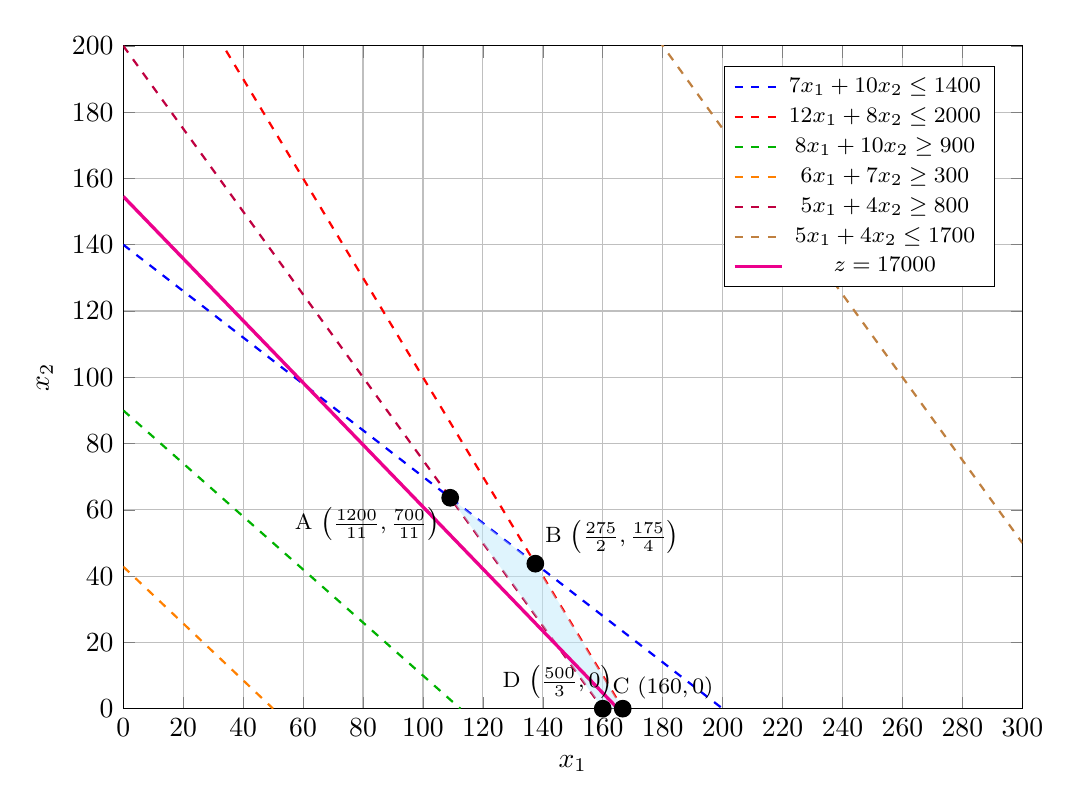
\begin{tikzpicture}
    \begin{axis}[
        xlabel={$x_1$},
        ylabel={$x_2$},
        xmin=0, xmax=300,
        ymin=0, ymax=200,
        grid=major,
        legend pos=north east,
        width=13cm,
        height=10cm,
        legend style={font=\footnotesize}
    ]
    
    % Restricción 1: 7x₁ + 10x₂ ≤ 1400 → x₂ ≤ 140 - 0.7x₁
    \addplot[blue, thick, dashed, domain=0:200] {140-0.7*x};
    \addlegendentry{$7x_1 + 10x_2 \leq 1400$}
    
    % Restricción 2: 12x₁ + 8x₂ ≤ 2000 → x₂ ≤ 250 - 1.5x₁
    \addplot[red, thick, dashed, domain=0:166.67] {250-1.5*x};
    \addlegendentry{$12x_1 + 8x_2 \leq 2000$}
    
    % Restricción 3: 8x₁ + 10x₂ ≥ 900 → x₂ ≥ 90 - 0.8x₁
    \addplot[green!70!black, thick, dashed, domain=0:112.5] {90-0.8*x};
    \addlegendentry{$8x_1 + 10x_2 \geq 900$}
    
    % Restricción 4: 6x₁ + 7x₂ ≥ 300 → x₂ ≥ 42.86 - 0.857x₁
    \addplot[orange, thick, dashed, domain=0:50] {(300/7)-(6/7)*x};
    \addlegendentry{$6x_1 + 7x_2 \geq 300$}
    
    % Restricción 5: 5x₁ + 4x₂ ≥ 800 → x₂ ≥ 200 - 1.25x₁
    \addplot[purple, thick, dashed, domain=0:160] {200-1.25*x};
    \addlegendentry{$5x_1 + 4x_2 \geq 800$}
    
    % Restricción 6: 5x₁ + 4x₂ ≤ 1700 → x₂ ≤ 425 - 1.25x₁
    \addplot[brown, thick, dashed, domain=0:300] {425-1.25*x};
    \addlegendentry{$5x_1 + 4x_2 \leq 1700$}
    
    % Región factible aproximada (necesitarías calcular los vértices exactos)
    % Esta es una aproximación visual de la región factible
    \fill[cyan!25, opacity=0.5] 
        (1200/11,700/11) -- (275/2,43.75) -- (500/3,0) -- (160,0) -- cycle;

    % Función objetivo
    \addplot[magenta, very thick, domain=0:165] {-(103/110)*x + (1700/11)};
    \addlegendentry{$z = 17000$}
    
    % Algunos puntos de intersección importantes (aproximados)
    \addplot[only marks, mark=*, mark size=3pt, color=black] 
    coordinates {(1200/11,700/11) (275/2,43.75) (500/3,0) (160,0)};
    
    % Etiquetas para algunos puntos clave
    \node at (axis cs:1200/11,700/11) [below left] {\footnotesize A \(\left(\frac{1200}{11},\frac{700}{11}\right)\)};
    \node at (axis cs:275/2,43.75) [above right] {\footnotesize B \(\left(\frac{275}{2},\frac{175}{4}\right)\)};
    \node at (axis cs:160,0) [above right] {\footnotesize C \(\left(160,0\right)\)};
    \node at (axis cs:500/3,0) [above left] {\footnotesize D \(\left(\frac{500}{3},0\right)\)};
    \end{axis}
    \end{tikzpicture}
    \caption{Región factible del PPL de ejemplo \ref{ej:modelo_de_ppl_verbal} en color \textcolor{cyan}{cyan}}
    \label{fig:ppl-maximizacion}
  \end{figure}
  Vemos que la la función objetivo \(z\) se encuentra dentro de la región factible, sin embargo, no es la solución óptima. Se puede ver que el punto más alejado del origen de coordenadas que puede tomar la función objetivo es el vértice \textit{B}. Por lo tanto, la solución óptima es el vértice \textit{B}, que es el punto \(\left(275/2,175/4\right)\). Entonces:
  \[
    z_B = 103\left(\frac{275}{2}\right) + 110\left(\frac{175}{4}\right) = \boxed{18975}
  \]

  \textbf{3. Respuesta:}

  En base a la resolución del PPL, se deben realizar \(137.5\) sesiones de destilación usando la tecnología nueva (\(T_n\)) y \(43.75\) sesiones de destilación usando la tecnología antigua (\(T_a\)), para obtener la mayor ganancia posible, que es \$\(18975\).

  \begin{tcolorbox}[remember]
    Aunque la respuesta pueda resultar confusa, recordemos que el enunciado decía que los procesos de destilación \textit{se pueden utilizar total o parcialmente}, por lo que la respuesta toma valores fraccionarios. Si se quisiera que la respuesta fuera un número entero, entonces se agregan las respectivas restricciones y se resuelve el PPL de la misma manera, tomando únicamente los puntos enteros de \(x_1\) y \(x_2\).
  \end{tcolorbox}

\end{quote}

\subsubsection{Método Simplex}

Como anteriormente mencionamos, el método simplex es un algoritmo que nos permite resolver problemas de optimización lineal. Aunque disponemos del método gráfico, cuando el número de \textit{variables de decisión} es grande (\(> 2\)), el método gráfico es impracticable, por lo que utilizar el método analítico se vuelve una necesidad.

Además, en general, la mayoría de los problemas de optimización suelen tener más de dos variables de decisión, por lo que la necesidad de generalizar la búsqueda de la solución optima es importante.

Antes de ver el método Simplex, vamos a ver algunos conceptos necesarios para comprender la formulación del método.

\paragraph{Forma matricial de un PPL}

Un PPL puede ser representado en forma matricial de la siguiente manera:
\begin{align*}
  \text{optimizar:} \quad   &z = \mathbf{c}^T\mathbf{x} \\[3pt]
  \text{sujeto a:} \quad    &A\mathbf{x} \thicksim  b \\
\end{align*}
donde:
\begin{itemize}
  \item \(\mathbf{c}\) es la matriz (o el vector) de coeficientes de la función objetivo
  \item \(\mathbf{x}\) es la matriz (o el vector) de variables de decisión
  \item \(A\) es la matriz de coeficientes de las restricciones
  \item \(b\) es la matriz (o el vector) de términos independientes de las restricciones
\end{itemize}
de forma explícita se puede ver como:
\begin{align*}
  \text{optimizar:} \quad   &z = c_{1}x_{1} + c_{2}x_{2} + \cdots + c_{n}x_{n} \\[3pt]
  \text{sujeto a:} \quad    &a_{11}x_{1} + a_{12}x_{2} + \cdots + a_{1n}x_{n} \thicksim b_{1} \\[3pt]
                            &a_{21}x_{1} + a_{22}x_{2} + \cdots + a_{2n}x_{n} \thicksim b_{2} \\[3pt]
                            &\quad \vdots \\[3pt]
                            &a_{m1}x_{1} + a_{m2}x_{2} + \cdots + a_{mn}x_{n} \thicksim b_{m} \\[3pt]
\end{align*}
\begin{align*}
  \text{donde:} \quad       &\mathbf{c} = \begin{pmatrix} c_1 \\ c_2 \\ \vdots \\ c_n \end{pmatrix},\ \mathbf{x} = \begin{pmatrix} x_1 \\ x_2 \\ \vdots \\ x_n \end{pmatrix},\ A = \begin{pmatrix} a_{11} & a_{12} & \cdots & a_{1n} \\ a_{21} & a_{22} & \cdots & a_{2n} \\ \vdots & \vdots & \ddots & \vdots \\ a_{m1} & a_{m2} & \cdots & a_{mn} \end{pmatrix},\ b = \begin{pmatrix} b_1 \\ b_2 \\ \vdots \\ b_m \end{pmatrix}
\end{align*}

Esta forma es conveniente ya que permite representar el PPL de una manera más compacta y permite referirnos a una parte específica como la matriz de los coeficientes \(\mathbf{c}\) para referirnos a los coeficientes de la función objetivo.

\paragraph{¿Qué necesitamos para usar el método Simplex?}

Para poder usar el método Simplex necesitamos, evidentemente un PPL, pero también necesitamos que el PPL esté en su \textit{forma estándar}. Un PPL está en su forma estándar si cumple determinadas condiciones:
\begin{enumerate}
  \item \textbf{Condición de no negatividad}: todas las variables de decisión deben ser positivas: \(\forall x_i,\ x_i \geq 0;\ i = 1,2,\ldots,n\)
  \item \textbf{Condición de restricciones}: todas las restricciones deben ser de la forma \(Ax = b\). Para lograr esto se introducen \hl{variables de holgura} y \hl{variables superfluas}.
\end{enumerate}
Estas dos condiciones consideran que \(b_i \geq 0\). Es decir, que todas las restricciones de la forma \(\sum a_{ij} x_{j} \thicksim b_i\), o bien de forma general:
\[
  a_{i1}x_1 + a_{i2}x_2 + a_{i3}x_3 + ... + a_{in}x_n \thicksim b_i
\]
tengan el término independiente \(b_i \geq 0\). Para lograr esto, si \(b_i < 0\), se multiplica toda la restricción por \(-1\).

Otra cosa que debemos tener es una \textbf{solución factible}, que llamaremos la \textit{solución factible inicial}. Esto es una solución que cumple con todas las restricciones y que, por lo tanto es factible, pero no necesariamente es la solución óptima. 

En algunos problemas, la solución factible inicial puede ser prácticamente trivial, es decir, que todas las variables de decisión sean cero, sin embargo, los ejemplos que hemos visto (ejemplo \ref{ej:resolucion_ppl_petroleos_grafico} y \ref{ej:mtd_grfico}) son problemas que no cumplen con esta condición, ya que \((0,0)\) no es una solución factible. 

\begin{tcolorbox}[interesting_data, title=Dato curioso]
  La caratula de este documento tiene un gráfico de un PPL que si tiene una solución factible inicial trivial, es decir, que todas las variables de decisión puedan ser cero. En el problema de la caratula, se busca maximizar \(z\), por lo que la solución factible inicial trivial no es la solución óptima, de hecho el beneficio para esa solución es \(z = 0\). 
\end{tcolorbox}

Esto lleva a que, en la mayoría de casos, encontrar una solución factible inicial no sea tan sencillo como lo parece, y por lo tanto, se tenga que buscar una a través de algún método o teorema. Esto lo profundizaremos más adelante, cuando hayamos visto cómo transformar un PPL en su forma estándar.

\paragraph{Transformación de un PPL en su forma estándar}

Como vimos anteriormente, Simplex requiere de un PPL en formato estándar. Si un PPL no cumple las dos condiciones del formato estándar, entonces debemos transformarlo a su forma estándar. 

Puede ver el siguiente video: \href{https://www.youtube.com/watch?v=6f5K3O7yUzU}{\texttt{forma estándar en programación lineal - YouTube}}, donde se muestran algunos ejemplos de cómo transformar un PPL a forma estándar. De igual manera, en este documento se mostrará el proceso de transformación a formato estándar de un PPL ejemplificado en dicho video. 

\ejemplo\label{ej:transformacion_ppl_forma_estandar}: Transformación de un PPL a forma estándar.

Consideremos el siguiente PPL (ejemplo del video recomendado):
\begin{align*}
  \text{maximizar:} \quad   &z = -8x_1 + 16x_2 - 4x_3 \\[3pt]
  \text{sujeto a:} \quad    &5x_1 + 8x_3 \geq 100 \\
                            &-x_1 + 6x_2 \geq 100 \\
                            &-6x_2 + 4x_3 \leq 100 \\
                            &x_1 \geq 0 \\
                            &x_2 \text{ Libre} \\
                            &x_3 \leq0
\end{align*}

\noindent\textbf{1. Condición de no negatividad:}

Este es un buen ejemplo ya que tenemos las tres posibilidades en las variables de decisión:
\begin{itemize}
  \item Libre: \(x_2\)
  \item Positiva: \(x_1\)
  \item Negativa: \(x_3\)
\end{itemize}

La única variable que cumple con la condición de no negatividad es \(x_1\), por lo tanto esta variable se mantiene como está, es decir, \(x_1 \geq 0\). 

Las variables que no cumplen con la condición de no negatividad son \(x_2\) y \(x_3\), por lo que debemos operar sobre ellas para hacer cumplir con la condición de no negatividad. Veamos el caso de \(x_3\) primero: 

La variable \(x_3\) es negativa, para transformar la restricción a positiva debemos realizar un cambio de variable, tal que:
\[
  x_3 = -y_3 \quad \rightarrow \quad y_3 \geq 0
\]

\noindent donde \(y_3\) es una variable que reemplaza a \(x_3\) y que es positiva. Esta variable debe cambiarse en todo el PPL, es decir, en la función objetivo y en las restricciones. 

Para el caso de \(x_2\), la variable puede tomar cualquier valor, por lo que para que estrictamente cumpla la condición de no negatividad podemos realizar lo siguiente:
\[
  x_2 = y_2 - y_2' \quad \rightarrow \quad y_2,\ y_2' \geq 0
\]

\noindent donde \(y_2\) y \(y_2'\) son variables que reemplazan a \(x_2\) y que cumplen con la condición de no negatividad. Estas variables deben reemplazar a \(x_2\) en todo el PPL, al igual que \(x_3\) se reemplaza por \(y_3\). Reemplazando las variables en el PPL, obtenemos:
\begin{align*}
  \text{maximizar:} \quad   &z = -8x_1 + 16y_2 - 16y_2' + 4y_3 \\[3pt]
  \text{sujeto a:} \quad    &5x_1 - 8y_3 \geq 100 \\
                            &-x_1 + 6y_2 - 6y_2' \geq 100 \\
                            &-6y_2 + 6y_2' - 4y_3 \leq 100 \\
                            &x_1,\ y_2,\ y_2',\ y_3 \geq 0
\end{align*}
Listo, la primer condición se cumple, ahora veamos la segunda condición.

\noindent\textbf{2. Condición de restricciones:}

La segunda condición es que todas las restricciones deben ser de la forma \(Ax = b\). En este caso, ninguna de las restricciones cumple con esta condición, por lo que debemos operar sobre todas ellas. 

Cuando analizamos la segunda condición, podemos encontrarnos con tres casos posibles:
\begin{enumerate}
  \item Restricción de la forma \(A_i x \leq b_i\): agregar una \textit{variable de holgura}
  \item Restricción de la forma \(A_i x \geq b_i\): agregar una \textit{variable superflua}
  \item Restricción de la forma \(A_i x = b_i\): cumple con la condición de forma estándar, por lo que no se necesita ninguna variable adicional
\end{enumerate}
\noindent donde \(A_i\) es la i-ésima restricción y \(b_i\) es su término independiente.
\begin{tcolorbox}[remember, title=¿Qué significa variable de holgura y variable superflua?]
  La \textbf{variable de holgura} es aquella que se agrega a una restricción de la forma \(A_i x \leq b_i\) para transformarla en una igualdad, y representa la cantidad de recursos de los que se disponían pero no se usaron. 

  \textit{Ejemplo}: si se disponen de 10 horas totales para fabricar un producto, pero solo se usan 8 horas, entonces la variable de holgura representa las \(2\) horas que se disponían pero no se usaron. 
  
  \vspace{3pt}

  Por otro lado, la \textbf{variable superflua} es aquella que se agrega a una restricción de la forma \(A_i x \geq b_i\) para transformarla en una igualdad, y representa la cantidad de recursos que se fabrican más de lo que se necesita.

  \textit{Ejemplo}: si se requieren como mínimo 54 toneladas de mineral, pero se extraen 60 toneladas, entonces la variable superflua vale \(60 - 54 = 6\) toneladas, y representa el exceso de toneladas de mineral que se extraen más de lo que se necesita. 
\end{tcolorbox}

\noindent Las restricciones de nuestro PPL que deben cumplir con esta condición son:
\begin{align*}
  5x_1 - 8y_3 &\geq 100 \\
  -x_1 + 6y_2 - 6y_2' &\geq 100 \\
  -6y_2 + 6y_2' - 4y_3 &\leq 100
\end{align*}
Para la tercera restricción, tenemos el caso 1. Para este caso debemos agregar una \textit{variable de holgura}:
\[
  -6y_2 + 6y_2' - 4y_3 \leq 100 \quad \rightarrow \quad -6y_2 + 6y_2' - 4y_3 + h_1 = 100
\]
Luego, para la primera y la segunda restricción tenemos el caso 2. Para este caso debemos agregar una \textit{variable superflua}:
\begin{align*}
  5x_1 - 8y_3 \geq 100 \quad &\rightarrow \quad 5x_1 - 8y_3 - s_1 = 100 \\
  -x_1 + 6y_2 - 6y_2' \geq 100 \quad &\rightarrow \quad -x_1 + 6y_2 - 6y_2' - s_2 = 100
\end{align*}

Estas variables que se han agregado a las restricciones deben aparecer en la función objetivo, sin embargo, como no son variables de decisión, su coeficiente en la función objetivo debe ser cero. Por lo que el PPL transformado a forma estándar es:
\begin{align*}
  \text{maximizar:} \quad   &z = -8x_1 + 16y_2 - 16y_2' + 4y_3 - 0s_1 - 0s_2 + 0h_1 \\[3pt]
  \text{sujeto a:} \quad    &5x_1 + 0y_2 - 0y_2' - 8y_3 - s_1 - 0s_2 + 0h_1 = 100 \\
                            &-x_1 + 6y_2 - 6y_2' + 0y_3 - 0s_1 - s_2 + 0h_1 = 100 \\
                            &0x_1 -6y_2 + 6y_2' - 4y_3 - 0s_1 - 0s_2 + h_1 = 100 \\
                            &x_1,\ y_2,\ y_2',\ y_3,\ h_1,\ s_1,\ s_2 \geq 0
\end{align*}
Si quitamos todos los términos con coeficiente nulo de las restricciones queda:
\begin{align*}
  \text{maximizar:} \quad   &z = -8x_1 + 16y_2 - 16y_2' + 4y_3 - 0s_1 - 0s_2 + 0h_1 \\[3pt]
  \text{sujeto a:} \quad    &5x_1 - 8y_3 - s_1 = 100 \\
                            &-x_1 + 6y_2 - 6y_2' - s_2 = 100 \\
                            &-6y_2 + 6y_2' - 4y_3 + h_1 = 100 \\
                            &x_1,\ y_2,\ y_2',\ y_3,\ h_1,\ s_1,\ s_2 \geq 0
\end{align*}

\paragraph{Generación de solución factible inicial}

Como vimos, Simplex también requiere de una solución factible inicial ya que el algoritmo se mueve de una solución factible básica a otra, mejorando el valor de la función objetivo en cada iteración. Entonces podemos generar una solución factible inicial a través de los siguientes métodos:
\begin{itemize}
  \item Inspección directa: si es fácil identificar un punto que satisface todas las restricciones, se puede usar directamente
  \item Método de la \textit{Fase I} del Simplex: para aquellos casos donde no es fácil aplicar la inspección directa, se utiliza este método. Este método consiste en cuatro pasos:
  \begin{enumerate}
    \item Se construye un problema auxiliar donde se agregan \textit{variables artificiales} para convertir el problema original en uno con una solución factible evidente
    \item Se minimiza la suma de esas variables artificiales
    \item Si en el óptimo esta suma es cero, se ha encontrado una solución factible al problema original
    \item Si no es cero, el problema original no tiene solución factible (es incompatible)
  \end{enumerate}
\end{itemize}

\subparagraph{Método de la Fase I}

Consiste en resolver un problema auxiliar con el único objetivo de encontrar una solución factible al problema original. Una vez que se obtiene dicha solución se procede a la \textit{Fase II} donde se busca la solución óptima del problema original.

Este método consiste en cuatro pasos:
\begin{enumerate}
  \item Transformar el problema a forma estándar
  \item Agregar variables artificiales en todas las restricciones que \textbf{no} se hayan agregado variables de holgura. En términos del PPL original podemos decir que se agrega una variable artificial en donde no se puede generar una solución factible inicial directa (restricciones del tipo \(\geq\) o \(=\)).
  \item Construir el problema auxiliar: el nuevo problema tiene como función objetivo minimizar la suma de las variables artificiales:
  \[\text{min}\ \omega = \sum_{i=1}^{n} a_i\]
  Esto se resuelve en el mismo método Simplex.
  \item interpretación del resultado: Si el valor óptimo es mayor que cero, el problema original no tiene solución factible (es incompatible). Si el valor óptimo es cero, entonces se ha encontrado una solución factible al problema original sin variables artificiales activas, por lo que se puede proceder a la Fase II.
\end{enumerate}

\ejemplo\label{ej:fase_1} El conjunto de restricciones:
\begin{quote}
  \begin{align*}
    x_1 + 2x_2 &\leq 3 \\
    4x_1 + 5x_2 &\geq 6 \\
    7x_1 + 8x_2 &= 15
  \end{align*}
  se transforma en un sistema de ecuaciones (forma estándar del PPL) agregando una variable de holgura \(h_1\) y una variable superflua \(s_1\):
  \begin{align*}
    x_1 + 2x_2 + h_1 &= 3 \\
    4x_1 + 5x_2 - s_1 &= 6 \\
    7x_1 + 8x_2 &= 15
  \end{align*}
  Si ahora se agregan respectivamente las variables artificiales \(a_1\) y \(a_2\), el problema auxiliar se transforma en:
  \begin{align*}
    x_1 + 2x_2 + h_1 \phantom{+ s_1 + a_1 + a_2} &= 3 \\
    4x_1 + 5x_2 \phantom{+ h_1} - s_1 + a_1 \phantom{+ a_2} &= 6 \\
    7x_1 + 8x_2 \phantom{+ h_1 - s_1 + a_1} + a_2 &= 15 \\
  \end{align*}
  Una solución \textit{no negativa} a este último sistema es:
  \begin{align*}
    h_1 &= 3 \\
    a_1 &= 6 \\
    a_2 &= 15 \\
    x_1 = x_2 = s_1 &= 0
  \end{align*}
  Nótese, sin embargo, que \(x_1=0\) y \(x_2=0\) no es una solución al conjunto inicial de restricciones. 
\end{quote}

\paragraph{Costos de Penalización}

La introducción de variables de holgura y superfluas no altera ni la naturaleza de las restricciones ni al objetivo. Por consiguiente, estas variables se incorporan a la función objetivo con coeficientes cero. Las variables artificiales, sin embargo, cambian la naturaleza de als restricciones. Ya que se agregan a un solo lado de una desigualdad, el nuevo sistema es equivalente al sistema anterior de restricciones sólo si las variables artificiales son cero. Para garantizar estas condiciones en la solución óptima las variables artificiales se introducen a la función objetivo con coeficientes muy grandes (si hay que maximizar la ganancia, una ganancia muy pequeña o negativa implica una gran penalización, por el contrario si hay que minimizar costos, un costo grande implica una gran penalización para esa variable). Estos coeficientes se denotan generalmente como \(+M\) (para minimización) o \(-M\) (para maximización).

Los coeficientes \(\pm M\) donde \(M\) se considera un número positivo muy grande, representan el severo costo de penalización que se impone a las variables artificiales cuando se activan en la solución óptima. 